%%%%%%%%%%%%%%%%%%%%%%%%%%%%%%%%%%%%%%%%%
% Beamer Presentation
% LaTeX Template
% Version 1.0 (10/11/12)
%
% This template has been downloaded from:
% http://www.LaTeXTemplates.com
%
% License:
% CC BY-NC-SA 3.0 (http://creativecommons.org/licenses/by-nc-sa/3.0/)
%
%%%%%%%%%%%%%%%%%%%%%%%%%%%%%%%%%%%%%%%%%

%----------------------------------------------------------------------------------------
%	PACKAGES AND THEMES
%----------------------------------------------------------------------------------------

\documentclass[hyperref={pdfpagemode=FullScreen},aspectratio=169]{beamer}
\setbeamertemplate{navigation symbols}{}

%This option causes the second screen to show the second mode material
\setbeameroption{second mode text on second screen=left}

\setbeameroption{show notes on second screen}

\mode<presentation> {

% The Beamer class comes with a number of default slide themes
% which change the colors and layouts of slides. Below this is a list
% of all the themes, uncomment each in turn to see what they look like.

%\usetheme{default}
%\usetheme{AnnArbor}
%\usetheme{Antibes}
%\usetheme{Bergen}
%\usetheme{Berkeley}
%\usetheme{Berlin}
%\usetheme{Boadilla}
%\usetheme{CambridgeUS}
%\usetheme{Copenhagen}
%\usetheme{Darmstadt}
%\usetheme{Dresden}
%\usetheme{Frankfurt}
%\usetheme{Goettingen}
%\usetheme{Hannover}
%\usetheme{Ilmenau}
%\usetheme{JuanLesPins}
%\usetheme{Luebeck}
\usetheme{Madrid}
%\usetheme{Malmoe}
%\usetheme{Marburg}
%\usetheme{Montpellier}
%\usetheme{PaloAlto}
%\usetheme{Pittsburgh}
%\usetheme{Rochester}
%\usetheme{Singapore}
%\usetheme{Szeged}
%\usetheme{Warsaw}

% As well as themes, the Beamer class has a number of color themes
% for any slide theme. Uncomment each of these in turn to see how it
% changes the colors of your current slide theme.

%\usecolortheme{albatross}
%\usecolortheme{beaver}
%\usecolortheme{beetle}
%\usecolortheme{crane}
%\usecolortheme{dolphin}
%\usecolortheme{dove}
%\usecolortheme{fly}
%\usecolortheme{lily}
%\usecolortheme{orchid}
%\usecolortheme{rose}
%\usecolortheme{seagull}
%\usecolortheme{seahorse}
%\usecolortheme{warsaw}
%\usecolortheme{whale}
%\usecolortheme{wolverine}
%\selectcolormodel{gray}

\setbeamercolor{normal text}{fg=white,bg=black!90}
\setbeamercolor{structure}{fg=white}
\setbeamercolor{alerted text}{fg=red!85!black}
\setbeamercolor{item projected}{use=item,fg=black,bg=item.fg!35}
\setbeamercolor*{palette primary}{use=structure,fg=structure.fg}
\setbeamercolor*{palette secondary}{use=structure,fg=structure.fg!95!black}
\setbeamercolor*{palette tertiary}{use=structure,fg=structure.fg!90!black}
\setbeamercolor*{palette quaternary}{use=structure,fg=structure.fg!95!black,bg=black!80}
\setbeamercolor*{framesubtitle}{fg=white}
\setbeamercolor*{block title}{parent=structure,bg=black!60}
\setbeamercolor*{block body}{fg=black,bg=black!10}
\setbeamercolor*{block title alerted}{parent=alerted text,bg=black!15}
\setbeamercolor*{block title example}{parent=example text,bg=black!15}

%\setbeamertemplate{footline} % To remove the footer line in all slides uncomment this line
%\setbeamertemplate{footline}[page number] % To replace the footer line in all slides with a simple slide count uncomment this line

%\setbeamertemplate{navigation symbols}{} % To remove the navigation symbols from the bottom of all slides uncomment this line
}

\usepackage{graphicx} % Allows including images
\usepackage{booktabs} % Allows the use of \toprule, \midrule and \bottomrule in tables
\usepackage[export]{adjustbox}
\usepackage{listings}
%----------------------------------------------------------------------------------------
%	TITLE PAGE
%----------------------------------------------------------------------------------------

\title[CCCamp]{A Geometry Engine from First Principles \\
               \large Three years into a six month project} % The short title appears at the bottom of every slide, the full title is only on the title page

\author{Julia Longtin} % Your name
\institute[HSlice] % Your institution as it will appear on the bottom of every slide, may be shorthand to save space
{
HSlice Project \\ % Your institution for the title page
\medskip
\textit{julia.longtin@gmail.com} % Your email address
}
\date{\today} % Date, can be changed to a custom date

% disable page count
\setbeamertemplate{page number in head/foot}{}

\begin{document}

\begin{frame}
  \titlepage % Print the title page as the first slide
  \begin{block}{Link to this talk}
    \begin{itemize}
    \item https://ni.faikvm.com/CCCamp2023.pdf
    \end{itemize}
  \end{block}
\end{frame}

%\begin{frame}
%\frametitle{Overview} % Table of contents slide, comment this block out to remove it
%\tableofcontents % Throughout your presentation, if you choose to use \section{} and \subsection{} commands, these will automatically be printed on this slide as an overview of your presentation
%\end{frame}

%----------------------------------------------------------------------------------------
%	PRESENTATION SLIDES
%----------------------------------------------------------------------------------------

%------------------------------------------------
\section{Who Am I?} % Sections can be created in order to organize your presentation into discrete blocks, all sections and subsections are automatically printed in the table of contents as an overview of the talk
%------------------------------------------------

\begin{frame}
  \frametitle{Who am I? (Role)}
  \begin{itemize}
  \item Free Software Developer
    \begin{itemize}
    \item Maintainer of ImplicitCAD
    \item Developer of HSlice
    \end{itemize}
  \item Work at Wire.com
    \begin{itemize}
    \item The presented work has no affiliation with my employer
    \end{itemize}
  \end{itemize}
  \note{Implicitcad is a 3d modelling system, and HSlice is the program i've been working on, that makes those models printable.}
  \note{Wire is an end-to-end encrypted communications platform. think: something like slack meets signal, but open source everything.}
\end{frame}

%------------------------------------------------

\begin{frame}
  \frametitle{Who am I? (???)}
  \begin{itemize}
  \item From Washington, DC.. and Northwest Arkansas.
  \item Have lived in Berlin with my wife for 4+ years.
  \item Transhumanist, Haskeller, CyberPunk enthusiast.
  \item Created a method for converting 3D prints to aluminium using microwaves (see: 31c3).
  \end{itemize}
  \note{I am from a very disadvantaged part of the united states, so have seen a lot of suffering which partially drives my work}
  \note{CyberPunk enthusiast is a polite way of saying I watch too much ghost in the shell, and spend too much time imagining how more technology could help both myself, and the people I care about.}
  \note{have some experience setting out to accomplish something really hard in the 3d printing world, which is what gave me the confidence to begin this project.}
\end{frame}

%------------------------------------------------

\section{Why Am I Here?}

%------------------------------------------------
\begin{frame}
  \frametitle{Why am I here?}
    I'm making a slicer!
  \begin{itemize}
  \item Hope:
    \begin{itemize}
    \item Hoping improving slicer technology can help people in the real world.
    \end{itemize}
  \item Inspiration:
    \begin{itemize}
    \item Glimmers of non-planar slicing in the 3D printing world.
    \end{itemize}
  \item Results I'm looking for (Better Slicers!):
    \begin{itemize}
    \item Parallelizing un-parallelized slicing algorithms.
    \item Increasing slicer precision.
    \item Increasing speed.
    \end{itemize}
  \end{itemize}
  \note{increased precision and increased speed is critical as we try to tackle more detailed prints made of more materials.}
\end{frame}

\subsection{Where I Began}

\begin{frame}
  \frametitle{Where I Began}
  \Huge{\centerline{What did I have before starting?}}
\end{frame}

\begin{frame}
  \frametitle{Status Quo}
  My 3d printing workflow:
  \begin{itemize}
  \item Open up a text editor, and describe my object.
  \item Hand it to my 3d modelling system.
  \item Wait.
  \item Receive an STL file. Open it in a visualizer, go back to step 1 if it's wrong.
  \item Open up a slicer, and hand it my STL file.
  \item Pick the material I want to use, and the quality level I want in the print.
  \item Wait.
  \item Receive a GCode file.
  \item Stick this file on a memory stick, and plug it into my printer.
  \item Wait.
  \item Receive a thing.
  \end{itemize}
  \note{I once waited 3 hours to slice a shoe in a single material.}
\end{frame}

\begin{frame}
  \frametitle{What is ImplicitCAD?}
  \begin{itemize}
  \item Programmatic 3D modelling system
  \item Written in Haskell
  \item Licensed under the AGPLv3+
  \end{itemize}
  \begin{block}{Online Editor}
    \begin{itemize}
    \item https://implicitcad.org/editor/
    \end{itemize}
  \end{block}
  \begin{block}{Source Code}
    \begin{itemize}
    \item https://github.com/Haskell-Things/ImplicitCAD/
    \end{itemize}
  \end{block}
\end{frame}

\begin{frame}
  \frametitle{What does ImplicitCAD do?}
  \begin{itemize}
  \item Reads and executes a program that uses Constructive Solid Geometry to describe objects.
  \item Renders 3D objects to files: STL, OBJ... ``Triangles on the outside''.
    \begin{itemize}
    \item Uses marching cubes algorithm for generating these triangles.
    \end{itemize}
  \item Highly parallelized, can utilize all CPUs
  \end{itemize}
  \begin{block}{Examples}
    \begin{itemize}
    \item https://www.implicitcad.org/examples
    \end{itemize}
  \end{block}
  \note{constructive solid geometry is a system of building up a complicated object from simpler parts. think: i need a plate, i need to subtract holes from it. i need to round the corners.. if you've used openscad, it's a subset of that language}
\end{frame}

\begin{frame}
  \frametitle{Current Slicers}
  \begin{itemize}
  \item Accept files containing 3D geometry: STL, OBJ... ``Triangles on the outside''.
  \item Output a simple file containing instructions for creating an object, for use by a 3D printer.
  \item Commonly use an external geometry engine (EG: openCASCADE).
  \end{itemize}
  Note: We're discussing FDM printing during this talk, but many other methods exist, each with their own plusses and minuses.
  \note{FDM is fused deposition of material... think, ``a hot glue gun on a robot''.}
\end{frame}

\begin{frame}
  \frametitle{What is a slicer's job?}
  We're going to use a basic definition.\par
  \par
  A slicer:
  \begin{itemize}
  \item Reads a file containing one or more objects.
    \begin {itemize}
    \item Objects are given as a series of triangles on the exterior of where the object begins.
    \end{itemize}
  \item Divides objects into layers.
  \item Writes instructions to fill in those layers. Different layer heights give different quality.
  \item Writes instructions to manage the non-geometry parts of 3D printing(temperature, speeds of movement, fan control..).
  \item Writes a GCode file contaiting these instructions, which can be given to a printer to produce the object(s) from the file.
  \end{itemize}
  \note{a pyramid could be represented as four triangles for what you see above the surface, and two in the base, making a square.}
  \note{GCode is basically instructions for ``go from point A to point B at speed X while extruding material at Y volume per second''}
\end{frame}

\section{Why do we need better slicers?}

\begin{frame}
  \frametitle{Why do we need better slicers?}
  \begin{itemize}
  \item Performance and Scalability(number of CPUs):
    \begin{itemize}
    \item Many slicers use geometry engines and algorithms that are single threaded..
    \item .. and are written in imperative languages.
    \item .. which hinders GPU, FPGA, or other accelerator usage.
    \end{itemize}
  \item Precision:
    \begin{itemize}
    \item Current major slicers use double precision floating point and linear algebra.
    \item Projective Geometry and more advanced algorithms can make use of the same double precision floating point, while introducing less error.
    \end{itemize}
  \item Scalability of printing:
    \begin{itemize}
    \item Models are getting more and more complex. we are learning to slice aross planes, to print with more materials at once, and are producing smaller objects (bioprinting, anyone?).
    \end{itemize}
  \end{itemize}
\end{frame}

\section{Inspiration}
\begin{frame}
  \frametitle{Inspiration: Non-Planar Printing}
  \begin{block}{University of Hamburg / Department of Informatics}
    \begin{itemize}
    \item https://youtu.be/km1lvuva5mI
    \end{itemize}
  \end{block}
  \note{https://youtu.be/km1lvuva5mI?t=100}
  \note{
    from talking about functionality to one implementation? two hard transitions.
    defining the geometry engine more explicitly. define what i'm talking about more upfront. makes explicit transitions better. re-examine the promise of exactly what's missing in the description. we're going to go deep into <x> algorithm, and explain how it works.
    insets broken in everything else. i can do better.
  }
  \note{I don't care if my slicer is the one we get to the destination with, i'm just trying to get us closer.}
\end{frame}

\section{First Decisions}

\begin{frame}
  \frametitle{Innovation Tokens}
  \Huge{\centerline{What did I think I would do differently?}}
\end{frame}

\begin{frame}
  \frametitle{Innovation Tokens}
  \begin{block}{Matthias Fischmann}
    Maintain a budget of innovation tokens. If you have to make an architectural decision (use servant, or write something nice ourselves? RIO or MTL, or write something nice ourselves?), you have to pay for choices that are more promising, but also more risky. If you are out of innovation tokens, you have to stick with what everybody else has been doing since forever.
  \end{block}

\end{frame}

\subsection{Innovations}

\begin{frame}
  \frametitle{Innovation Token 1: Using Haskell}
  \begin{itemize}
  \item A Functional programming language.
  \item Lazy:
    \begin{itemize}
    \item Does not perform an operation until its needed.
    \end{itemize}
  \item Separates Pure from Impure code:
    \begin{itemize}
    \item Pure code does not retain state between function calls.
    \item Pure code is simpler to parallelize, simpler to test.. 
    \item .. and possible to port to FPGAs / GPUs.
    \end{itemize}
  \end{itemize}
  \note{Coding in pure Haskell is more like writing math. you don't give your compiler a sequence of instructions, you give a big formula, describing the relationship between your problems. this gives the compiler more opportunities to try to out-think you, and to optimize your code.}
\end{frame}

\begin{frame}
  \frametitle{Innovation Token 2: Building my own geometry engine}
  \begin{itemize}
  \item Not using the giant geometry libraries from the 80s.
  \item Allows the use of more advanced algorithms and algebras..
  \item Avoided interfacing with non-Haskell code:
    \begin{itemize}
    \item Allows for knowing what parts of the library (all of them!) are Pure code.
    \item Allows easier parallelization, refactoring.
    \end{itemize}
  \end{itemize}
  \note{I implemented this progressively, writing the parts I needed, as I needed them.}
\end{frame}

\begin{frame}
  \frametitle{Innovation Token 3: Using Projective Geometric Algebra}
  \begin{itemize}
  \item uses one more parameter for each of it's primitives:
    \begin{itemize}
    \item 2D Points are represented using three values.
    \item 2D Lines are represented using three values.. and are not line segments.
    \end{itemize}
  \end{itemize}
  Inspiration:
  \begin{block}{SIGGRAPH2019 - Geometric Algebra for Computer Graphics - Charles Gunn and Steven De Kennick}
    https://youtu.be/tX4H\_ctggYo
  \end{block}
  \begin{itemize}
  \item ``Geometric Algebra is like Functional programming for linear algebra. Mindblowing.'' - @henrmota
  \end{itemize}
  \note{We are using a clifford algebra of (2,0,1)*}
\end{frame}

\begin{frame}
  \frametitle{Innovation Token 4: New Geometry Algorithms}
  \begin{itemize}
  \item Faster algorithms available.
  \item Parallelism? I think so...
  \end{itemize}
\end{frame}

\section{How I Got Here}

\begin{frame}
  \frametitle{Beginning Work}
  \Huge{\centerline{How did I get started?}}
\end{frame}

\begin{frame}
  \frametitle{By NOT starting from scratch}
  \begin{block}{Catherine Moresco and Noah Halford - Slicer(Whack?)}
    https://github.com/nhalford/slicer
  \end{block}
  What That Got Me:
  \begin{itemize}
  \item A Slicer!
    \begin{itemize}
    \item With basic linear algebra..
      \begin{itemize}
      \item Based on euclidian points, 2D line segments.
      \end{itemize}
    \item One test case, with no reference for what it should produce...
    \item Filled in layers of a print, as long as they had only convex angles at their exterior nodes..
    \end{itemize}
  \end{itemize}
  \note{the first mistake I think most developers make is assuming no-one has tried what you're trying to do.}
  \note{our definition of convex: If you put a baloon around it, the baloon would touch all of the line segments.}
\end{frame}

\begin{frame}
  \frametitle{Spending our Innovation Tokens}
  \Huge{\centerline{How did it go?}}
\end{frame}

\begin{frame}
  \frametitle{Experience of only using Haskell}
  As I have maintained ImplicitCAD for many years, Haskell generally got ``out of my way'', with the following exceptions:
  \begin{itemize}
  \item Floating point rounding control is a separate library, which seems un-loved, and does not work on GHC 9.2 yet.
  \item There is always a better way to learn to do things in Haskell, which led to me having many moments of ``who wrote this crap?'' as I re-factored over the years.
  \item The compiler and type system worked closely with me, when refactoring! :)
  \item When implementing a function where I didn't know how to handle all of the possible cases, I could set up a filter, and call error() in the cases I don't know how to implement yet.
  \end{itemize}
\end{frame}

\begin{frame}
  \frametitle{Experience of adding Geometric Algebra}
  We needed a Geometric Algebra library, to do the math for Projective Geometric Algebra functions.\par
  A Geometric Algebra is a system of algebra operating on values in vector spaces. \par
  Think: Number plus axis, where we have a lot of axises, and combinations of axises.
  \begin{itemize}
  \item The papers I was using did not define in detail the operators they were using, which slowed development. The word 'multiply' had a lot of meanings.
    \begin{itemize}
    \item It took quite some time to determine how to perform the operations described.
    \item Then I had to learn how to abuse sort() for performing reduction of geometric products.
    \item Finally, I learned the hard way that i needed to treat scalars as their own axis in the geometric product.
    \item .. I still don't have the math for the origin working right. avoid (0,0). :)
    \end{itemize}
  \end{itemize}
  \note {I am no mathematician}
  \note {somehow, I ended up with three operators, which when used together, do the work of the two sub operators they defined (wedge and dot product).}
\end{frame}

\begin{frame}
  \frametitle{Resources to prevent the same mistakes}
  \begin{block}{BiVector.net: 2D Projective Geometric Algebra Cheat Sheet}
    https://bivector.net/2DPGA.pdf
  \end{block}
  \begin{block}{My Code! :)}
    github.com/Haskell-Things/HSlice/blob/master/Graphics/Slicer/Math/GeometricAlgebra.hs
  \end{block}
\end{frame}

\begin{frame}
  \frametitle{Experience of adding Projective Geometric Algebra}
  Long and painful. Arguably incomplete in the error estimation area.
  \begin{itemize}
  \item There are many papers by Charles Gunn, which assume a level of math I'm not at.
    \begin{itemize}
    \item The symbols used in many places are not defined.
    \item Normalization and canonicalization were new concepts to me. ``you mean, after some operations, you have to perform a specific operation on the result so other operations work correctly?''
    \item Normalization and canonicalization are necesary.. sometimes. They are often skipped in the papers. It took much trial and error to find the right places to perform each operation.
    \end{itemize}
  \item Using the type system of haskell to only normalize and canonicalize when necessary was necessary so as to not accidentaly throw away precision and performance.
  \item Finding symmetry breaking operations took work. Some of the operations you need when reasoning about geometry were not well documented.\par
    Think: ``if I compare line A to line B, does line A point toward the left/right/forward/backward compared to line B?''
  \end{itemize}
\end{frame}

\begin{frame}
  \frametitle{Resources to prevent the same mistakes}
  \begin{block}{Charles G. Gunn: Projective Geometric Algebra}
    https://arxiv.org/pdf/1901.05873.pdf
  \end{block}
  \begin{block}{BiVector forum Projective GA category}
   https://discourse.bivector.net/c/projective-ga/
  \end{block}
  \begin{block}{My Code! :)}
    github.com/Haskell-Things/HSlice/blob/master/Graphics/Slicer/Math/PGAPrimitives.hs
  \end{block}
\end{frame}

\begin{frame}
  \frametitle{Experience of adding new geometry algorithms}
  Longer, and painfuller. Had to learn about a part of math I hadn't even heard of before: Straight Skeleton Generation.\par
  Implementation is incomplete. Just starting to slice complicated shapes, no hole handling yet.
  \begin{itemize}
  \item Straight Skeletons are deceptively simple. I estimated difficulty without even understanding this part.
  \item Many papers have been written on the subject, but very few have implementations.. and none have Haskell implementations.
  \item The mathematical approach of measuring algorithmic speed does not fit well with our modern multi-core world.
  \item I found one paper that's approachable.. but still have not implemented it completely.
  \end{itemize}
  \note{If it is less steps, but requires a single fast core.. it will run horribly on modern computers.}
\end{frame}

\begin{frame}
  \frametitle{Resources to prevent the same mistakes}
    \begin{block}{Christopher Tscherne - Straight Skeletons \& Motorcycle Graphs}
      https://diglib.tugraz.at/download.php?id=5c4a4913a9ed9\&location
    \end{block}
    This Talk? :)
\end{frame}

\begin{frame}
  \frametitle{Results}
  \Huge{\centerline{What did that get us?}}
\end{frame}

\begin{frame}
  \frametitle{HSlice!}
  A Haskell based slicer!
  \begin{itemize}
    \item A Geometric Algebra library!
      \begin{itemize}
      \item With Floating Point error tracking.
      \end{itemize}
    \item A mixed Euclidian / Projective geometry engine.
      \begin{itemize}
      \item With a large (260 at present) test suite.
      \end{itemize}
    \item A Parallel Straight Skeleton solver.
    \item A binary styled after the Cura slicing engine.
    \item Just a hair more precision..
  \end{itemize}
  \note{naming is hard, so i didn't try.}
  \note{if i slice with exactly the same settings and features between my slicer and cura, i save just a touch of plastic, because the lines are straighter, and less floating point error makes it into the print.}
\end{frame}

\begin{frame}
  \frametitle{Results}
  \Huge{\centerline{So what is a Straight Skeleton,}}\par
  \Huge{\centerline{and why do we need to solve it?}}
\end{frame}

\begin{frame}
  \frametitle{Visualizing Geometry}
  For drawing the figures for the rest of the talk, we're going to use:
  \begin{block}{Ganja.JS}
    https://enkimute.github.io/ganja.js/
  \end{block}
  \note{weaknesses of ganja.js: always focuses on the origin, no ray primitive, labels for two points at the same point overwrite each other.}
\end{frame}

\subsection{Adding Slicing Primitives}

\begin{frame}
  \frametitle{Rendering a Triangle}
    \includegraphics[width=0.9\textwidth, center]{triangle\-Straight_Skeleton.png}
  \note{Point out the exterior nodes, and the interior node.}
\end{frame}

\begin{frame}
  \frametitle{Slicing Primitives: Contour}
  \begin{itemize}
  \item A sequence of at least three line segments.
  \item Closed.
  \item Only two line segments end/start at any point.
  \item No line segments intersect any other line segment, except at their end/start point.
  \item Interesting Attributes:
    \begin {itemize}
      \item Has a winding, clockwise or counterclockwise.
    \end{itemize}
  \item Interesting Operations:
    \begin {itemize}
    \item outset: to draw a bigger form of the contour where each line segment is a given distance from its companion in the original contour.
    \item inset: to draw a smaller form of the contour where each line segment is a given distance from its companion in the original contour.
    \end{itemize}
  \end{itemize}
  \note{weaknesses of ganja.js: always focuses on the center, no ray primitive, labels at the same point collide.}
\end{frame}

\begin{frame}
  \frametitle{Slicing Primitives: Exterior Nodes}
  \begin{itemize}
  \item Exist at the point two line segments intersect forming a concave angle from the perspective of the inside of the contour.
  \item Always emit a ray toward the inside of the contour, along the bisector of the angle created by the two line segments.
  \end{itemize}
\end{frame}

\begin{frame}
  \frametitle{Slicing Primitives: Interior Nodes}
  \begin{itemize}
  \item Exist at the point that rays meet inside of a contour.
  \item Always emit a ray away from the input rays, along the bisector of the input rays(in the concave case).
  \end{itemize}
  \note{interior nodes are the joints in our straight skeleton}
\end{frame}

\subsection{Inset, Outset, and Straight Skeletons}

\begin{frame}
  \frametitle{What are insets and outsets?}
  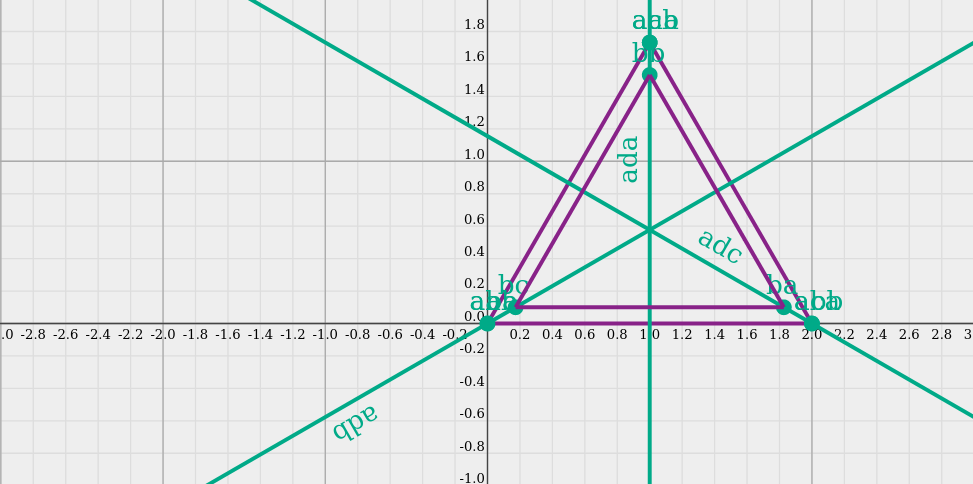
\includegraphics[width=0.9\textwidth, center]{triangle-one_inset.png}
\end{frame}

\begin{frame}
  \frametitle{Insets: Always on the Straight Skeleton}
    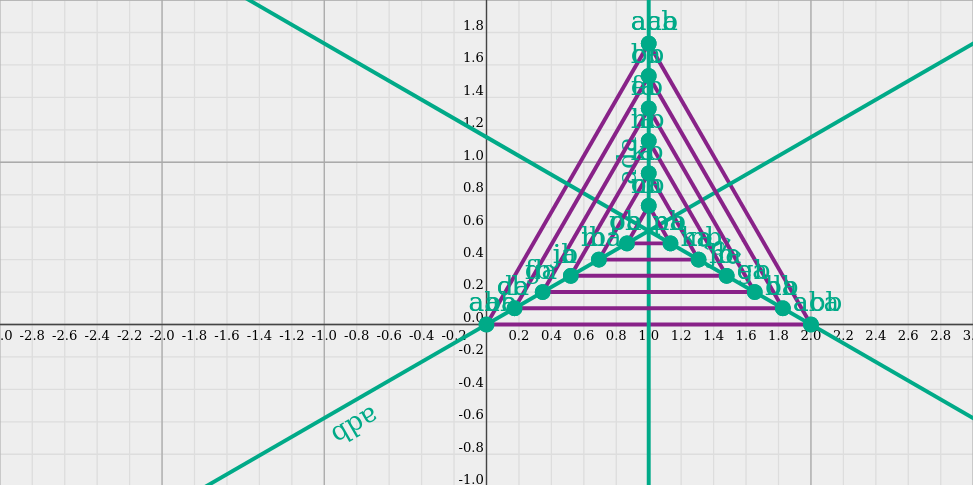
\includegraphics[width=0.9\textwidth, center]{triangle-all_insets.png}
\note{straight skeleton: the line segments on which we start and stop our inset line segments we are drawing the inset an object}
\end{frame}

\begin{frame}
  \frametitle{More Insets: Square}
    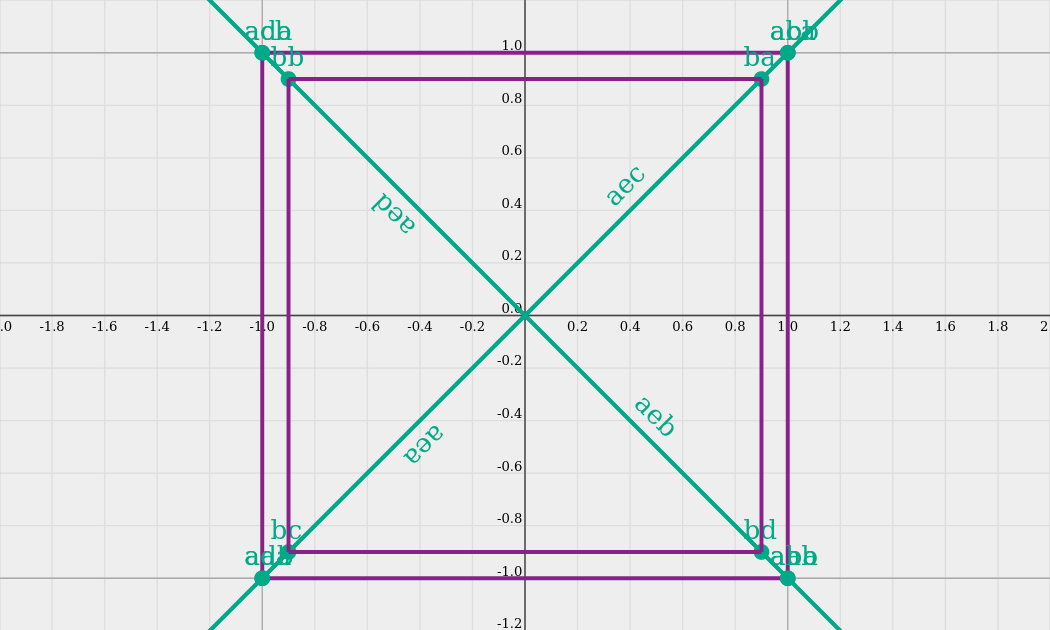
\includegraphics[width=0.7\textwidth, center]{square-Straight_Skeleton_and_Inset.png}
\end{frame}

\begin{frame}
  \frametitle{More Insets: Square}
    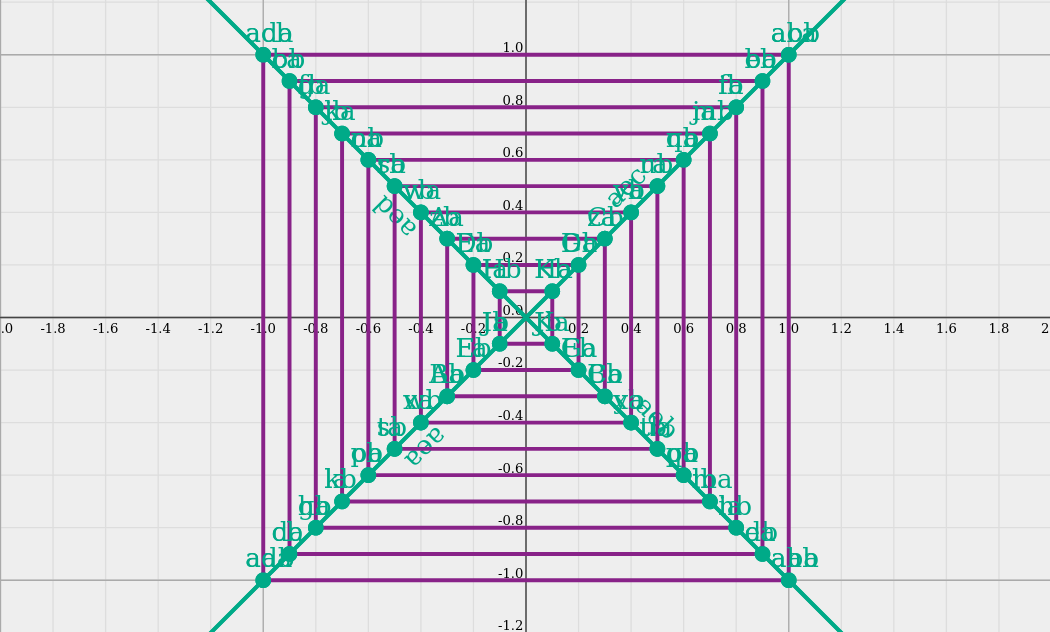
\includegraphics[width=0.7\textwidth, center]{square-Straight_Skeleton_and_Insets.png}
\end{frame}

\begin{frame}
  \frametitle{Straight Skeletons}
  \Huge{\centerline{Why is any of this complicated?}}
\end{frame}

\begin{frame}
  \frametitle{More Insets: Rectangle}
  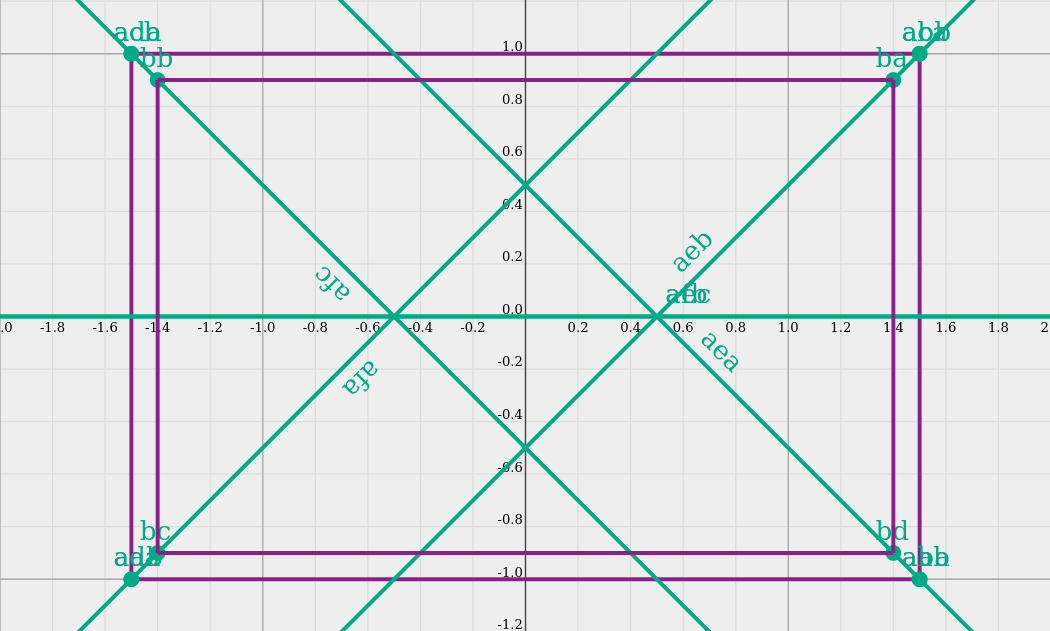
\includegraphics[width=0.7\textwidth, center]{rectangle-Straight_Skeleton_and_Inset.png}
  \note{hslice's geometry engine is written to generate straight skeletons, for the purpose of doing insets and outsets.}
\end{frame}

\begin{frame}
  \frametitle{Drawing the Straight Skeleton of a Convex Contour}
  \begin{itemize}
  \item Examine the collision of all of the rays emitted from nodes in the object.
  \item Determine the collision that has the shortest distance from its input nodes.
  \item Remove the input nodes from your list to be searched, and replace it with an interior node.
    \begin{itemize}
    \item for two input nodes output of this new interior node will be anticollinear with the bisector of the input nodes.
    \end{itemize}
  \item Wash, Rinse, Repeat.
  \end{itemize}
    \note{repeat: our definition of convex: If you put a baloon around it, the baloon would touch all of the line segments.}
    \note{go back to the last slide, and solve it in-front of everyone}
\end{frame}

\subsection {Solving a simple Division}

\begin{frame}
  \frametitle{What to do here?}
  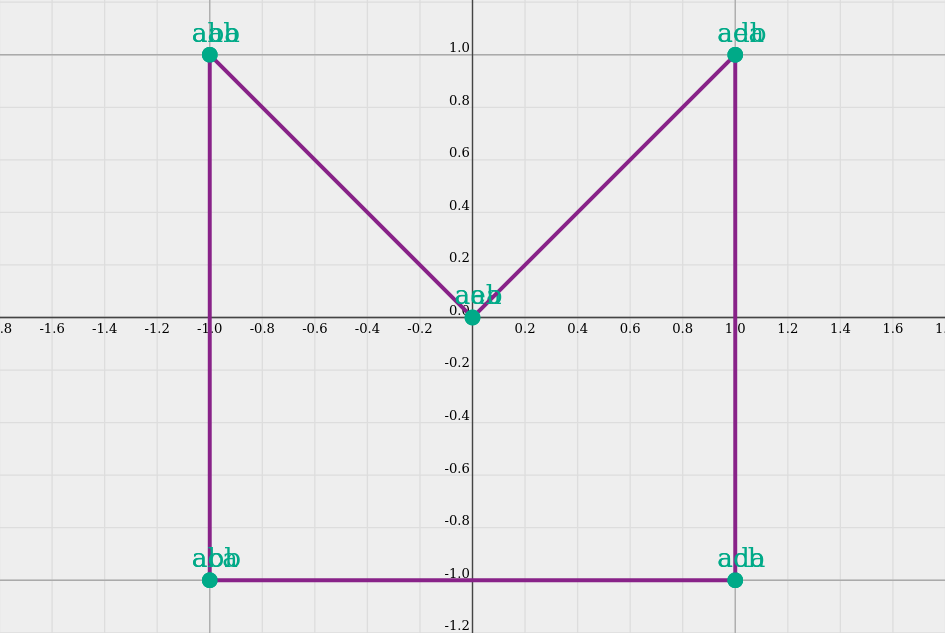
\includegraphics[width=0.68\textwidth, center]{C3.png}
  \note{Explain basically what a motorcycle is here. repeat our definition of convex.}
\end{frame}

\begin{frame}
  \frametitle{Removing the Noise}
  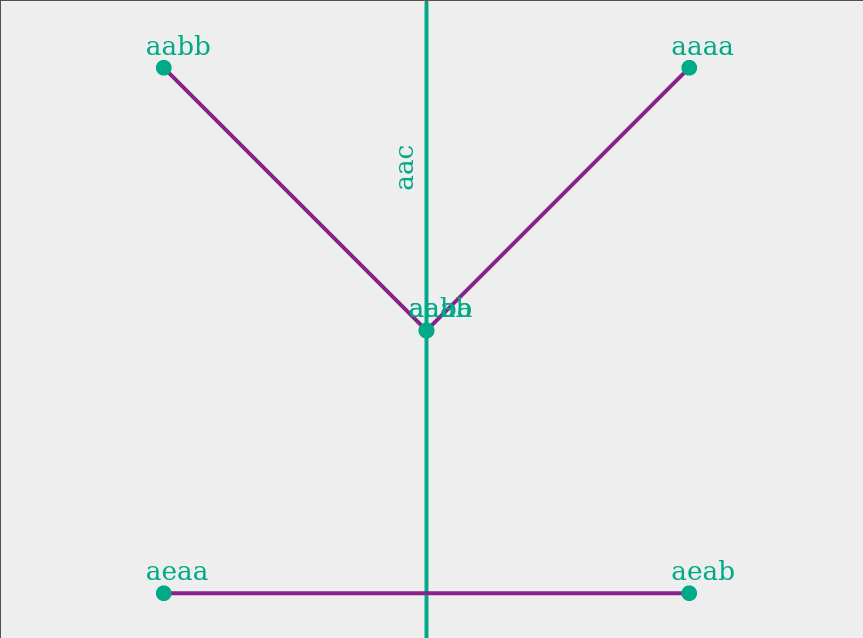
\includegraphics[width=0.6\textwidth, center]{C3-motorcycle-nogrid.png}
  \note{Explain what we have removed, and what remains}
\end{frame}

\begin{frame}
  \frametitle{Slicing Primitives: Motorcycles}
  \begin{itemize}
  \item Emitted from at the point two line segments intersect forming a convex angle from the perspective of the inside of the contour.
  \item Can collide with an exterior line, an exterior node, or another motorcycle.
  \item for a motorcycle that does not hit another motorcycle, the point the straight skeleton passes through the motorcycle, and the lines the skeleton must enter/exit are calculable.
  \item Interesting Attributes:
    \begin {itemize}
      \item Has a speed (speeding motorcycles!).
    \end{itemize}
  \end{itemize}
  \note{speeding motorcycles are impossible to search for.}
\end{frame}

\begin{frame}
  \frametitle{Speeds}
  \begin{itemize}
  \item Motorcycle Speed: The distance along the motorcycle between the point the motorcycle is emitted, and where it would intersect with a line that is parallel to, and one unit away from one of the motorcycle's input lines segments.
  \item Wall Collision Speed: The distance along the motorcycle between the point the motorcycle hits the wall, and where it would intersect with a line that is parallel to, and one unit away from the wall.
  \end{itemize}
  \note{So, in the case of being emitted from a 90 degree angle, we use asquared + bsquared = csquared, which gives us a speed of 1.41.}
\end{frame}

\begin{frame}
  \frametitle{Finding the Crossover Point}
  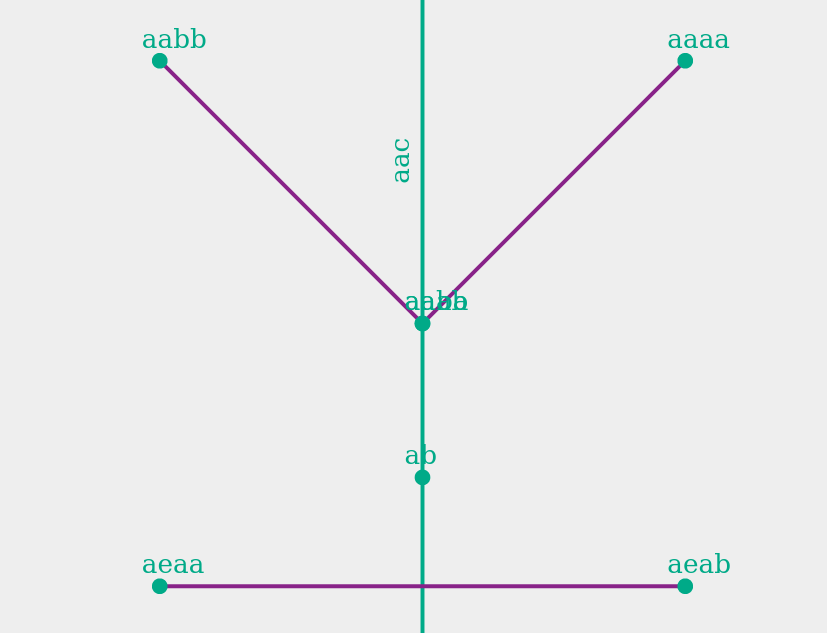
\includegraphics[width=0.55\textwidth, center]{C3-motorcycle-point-nogrid.png}
  \note{sqrt (2) == 1.41, multiply the two points, then add.}
\end{frame}

\begin{frame}
  \frametitle{Finding the Crossover Point}
  The crossover point is the point which the straight skeleton must pass through between two cells.\par
  To find the crossover point:
  \begin{itemize}
  \item Determine the speed of the emitted motorcycle.
  \item Determine the speed of the object it collided with.
  \item Place a point along the motorcycle where the ratio of the distance between the base of the motorcycle and the point of impact has the same ratio as the speeds do.
  Example:
    \begin{itemize}
    \item For the last shown object, the motorcycle is emitted from a 90 degree angle.
    \item a line parallel to one of it's input line segments and 1 unit away would cross the motorcycle sqrt(2), or ~1.41 units away, giving it a speed of ~1.41.
    \item a the wall intersected is at a 90 degree angle to the motorcycle, so would have a speed of 1.
    \item so the distance between the motorcycle base and the point is 1.41 times the distance between the point and where the motorcycle intersects the target line.
    \end{itemize}
  \end{itemize}
\end{frame}
    
\begin{frame}
  \frametitle{Finding a Crossover Line}
  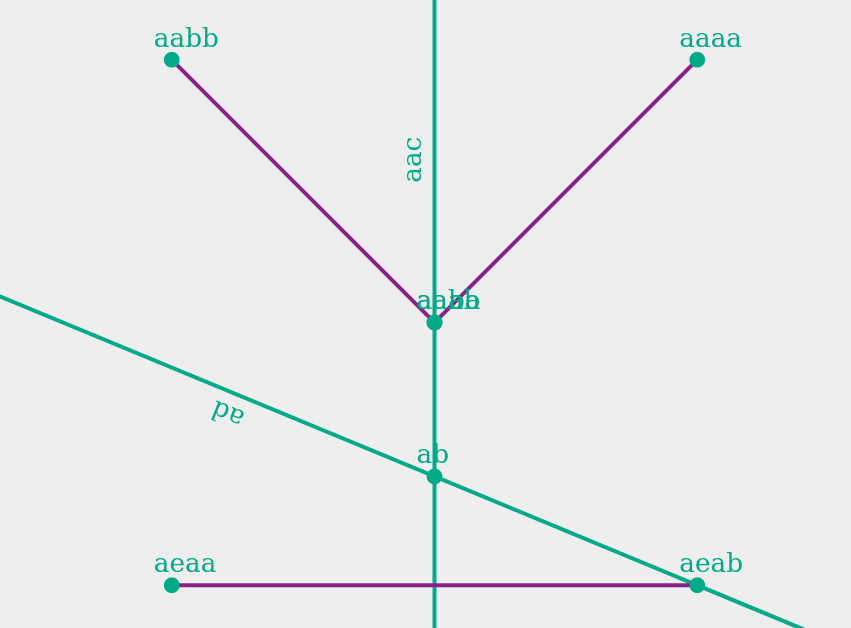
\includegraphics[width=0.6\textwidth, center]{C3-motorcycle-left_line-nogrid.png}
  \note{sqrt (2) == 1.41, multiply the two lines, then add.}
\end{frame}

\begin{frame}
  \frametitle{Finding the Crossover Line}
  The crossover lines are the lines which the straight skeleton must pass through on both sides of our crossover point.\par
  To find the crossover line:
  \begin{itemize}
  \item Determine the speed of the emitted motorcycle.
  \item Determine the speed of the object it collided with.
  \item Place a line where the ratio of the distance between the line segment on that side of the motorcycle and the line it impacts has the same ratio as the speeds do.
  Example:
    \begin{itemize}
    \item For the last shown object, the motorcycle is emitted from a 90 degree angle.
    \item a line parallel to one of it's input line segments and 1 unit away would cross the motorcycle sqrt(2), or ~1.41 units away, giving it a speed of ~1.41.
    \item a the wall intersected is at a 90 degree angle to the motorcycle, so would have a speed of 1.
    \item so the distance between the motorcycle base and the new line is 1.41 times the distance between the new line and where the motorcycle intersects the target line.
    \end{itemize}
  \end{itemize}
\end{frame}

\begin{frame}
  \frametitle{Implications?}
  \begin{itemize}
  \item Because the crossover point and lines can be calculated directly from just the input segments of the motorcycle, and the object collided with:
    \begin {itemize}
    \item we can calculate the straight skeletons of the two sides separately, giving us multiple cells. Parallelism, and reduced work on both sides!
    \item when calculating using cells, error in calculation is not propogated across the divide.
    \end {itemize}
  \item Because PGA has operations for both finding a point at a ratio between two points, and for finding a line at a ratio between two other lines, The crossover finding functions are easy to implement.
  \item Crossover calculations do not work if one of the interior nodes of the skeleton of one side crosses over to the other side. for this situation, see Christopher Tscherne's paper referenced earlier.
  \end {itemize}
\end{frame}

\subsection{Adding Projective Geometric Algebra}

\begin{frame}
  \frametitle{Slicing Primitives: Cells}
  \begin{itemize}
  \item Have a non-zero number of sides, composed of multiple connected line segments.
  \item are separated from other cells by motorcycles.
  \end{itemize}
\end{frame}

\begin{frame}
  \frametitle{Projective Geometric Algebra}
  \Huge{\centerline{How does PGA help?}}
\end{frame}

\begin{frame}
  \frametitle{PGA Primitives: 2D Projective Point}
  \begin{itemize}
  \item Based on values in three basis vectors pairs:
    \begin {itemize}
    \item (e0, e1)
    \item (e0, e2)
    \item (e1, e2)
    \end{itemize}
  \item Interesting Operations:
    \begin {itemize}
    \item add two points: get a point in-between them
    \item multiply both points by values a,b, then add them: get a point a/b between the two points
    \item multiply two points: get a line between them, and the distance between the points
    \end{itemize}
  \end{itemize}
\end{frame}

\begin{frame}
  \frametitle{PGA Primitives: 2D Projective Line}
  \begin{itemize}
  \item Based on values in three basis vectors:
    \begin {itemize}
    \item e0 -- TranslationISH
    \item e1 -- xInterceptISH
    \item e2 -- yInterceptISH
    \end{itemize}
  \item Interesting Operations:
    \begin {itemize}
    \item add two lines: get the line in-between them
    \item multiply both lines by values a,b, then add them: get a line a/b between the two lines
    \item no e1? parallel to the X axis.
    \item no e2? parallel to the Y axis.
    \item use the translationISH and an interceptISH to get a real intercept.
    \end{itemize}
  \item Interesting Properties:
    \begin {itemize}
    \item Has a direction.
    \end{itemize}
  \end{itemize}
\end{frame}

\begin{frame}
  \frametitle{Projective Geometric Algebra}
  \Huge{\centerline{What about floating point error?}}
\end{frame}

\subsection{Floating Point Pain}
\begin{frame}
  \frametitle{Floating Point and Projective Geometric Algebra}
  \begin{itemize}
  \item We implemented PGA using IEEE754 double precision.
    \begin {itemize}
    \item One sign bit.
    \item 11 exponent bits.
    \item 52 fraction bits.
    \end{itemize}
  \item X86 has three multiply modes:
    \begin {itemize}
      \item Give me the closest answer above the 'real' answer.
      \item Give me the closest answer to the 'real' answer.
      \item Give me the closest answer below the 'real' answer.
    \end{itemize}
  \item Unit of Least Precision:
    \begin {itemize}
    \item the least significant bit of a value.
    \end{itemize}
  \end{itemize}
\end{frame}

\begin{frame}
  \frametitle{Acquiring Error Bars}
  \begin{itemize}
  \item Every time you perform a calculation:
    \begin {itemize}
      \item Get the closest answer to the 'real' answer.
      \item Get the closest answer above the 'real' answer.
      \item store the closest answer to the 'real' answer.
      \item store the unit of least precision of the closest answer above the 'real' answer.
    \end{itemize}
  \end{itemize}
\end{frame}

\begin{frame}
  \frametitle{Utilizing Error Bars}
  \begin{itemize}
  \item Every time you perform a geometric operation, take into account these errors:
    \begin {itemize}
    \item Comparing where a line intersects with the end of a line segment?
      \begin {itemize}
      \item Use the ULP(Unit of Least Precision)s to decide on the size of a 'hit circle' around the endpoint
      \item Check distance of the found intersection from that point.
      \item Intersections between two line segments at the same point will probably have different sized hit circles!
      \end{itemize}
    \item Checking whether two lines are collinear?
      \begin {itemize}
      \item Use the ULPs to decide on the size of deviation that's possible.
      \end{itemize}
    \item EACH situation may have different ways to interpret!
    \item When in doubt, add a fudge multiplier, and think through your operations!
    \end{itemize}
  \end{itemize}
  \note { define a ULP here}
\end{frame}

\begin{frame}
  \frametitle{Total Cheating}
  \begin{itemize}
  \item Abusing Laziness:
    \begin{itemize}
    \item Haskell is a lazy language.
    \item ULPs allow you to find error bars, including error amounts that might be undesireable.
    \item Solution? tell the compiler to the calculation in a fixed point library, and de-reference it when error is too high!
    \end{itemize}
  \end{itemize}
\end{frame}

\subsection{Property Testing}

\begin{frame}
  \frametitle{Property Tests}
  \Huge{\centerline{How do I know any of that worked?}}
\end{frame}

\begin{frame}
  \frametitle{Property Tests}
  Property tests test for a ``property'' of calling a function with random data.
  \par Examples:
  \normalsize
  \begin{itemize}
    \item unit test: 2 `add` 2 == 4
    \item property test: a `add` b \textgreater a \par where a,b :: (Positive Integer)
    \item property test: a `add` b \textgreater b \par where a,b :: (Positive Integer)
    \item property test: a `add` b \textless b*2 \par where a,b :: (Positive Integer) and a \textless b
  \end{itemize}
\end{frame}

\begin{frame}
  \frametitle{Property Testing Geometry}
  \large To property test geometry, you must do a few things:
  \begin{itemize}
  \item Create a function from a set of (radian, distance) and a center point to a contour.
  \item Call that function from your property test, and test properties!
  \item Think:
    \begin{itemize}
    \item the point of the interior node of a triangle is always inside the triangle..
    \item a square always has one interior node.
    \item a rectangle always has two interior nodes.
    \item an inset unit polygon retains the number of exterior nodes as it shrinks.
    \end{itemize}
  \end{itemize}
  \begin{block}{Idea Stolen From:}
    https://stackoverflow.com/questions/8997099/algorithm-to-generate-random-2d-polygon
  \end{block}
\end{frame}

\begin{frame}
\frametitle{-Fin-}
\Huge{\centerline{Questions?}}
\large{email: julia.longtin@gmail.com}
\end{frame}

%\subsection {tscherne's algorithm}
%\subsection {Cells with holes}

%\note{< geekosaur> one small difference: rather than using `error` directly I used a synonym, so I could see which use sites were incomplete vs. expected error cases}

%------------------------------------------------
%\begin{block}{Source to this talk}
%\begin{itemize}
%\item https://github.com/julialongtin/CCCamp2023.git
%\end{itemize}
%\end{block}

\end{document}
